\chapter{संकुलन}\label{ch:b1:complexation}

हल्के नीले कॉपर(II) सल्फ़ेट में थोड़ा अमोनिया विलयन डालिए: तुरंत एक हल्का
नीला अवक्षेप बनता है। और डालिए, तो अवक्षेप घुलकर गहरे, लगभग स्याही जैसे
नीले रंग का विलयन बन जाता है। अम्ल--क्षारक या अवक्षेपण के अध्यायों में कुछ भी
दूसरे चरण की व्याख्या नहीं करता। अमोनिया के अणु अपने \omterm{def:b1:lewis-resonance-vsepr:lewis}{एकाकी युग्मों} द्वारा
कॉपर आयन से बँध गए हैं और उन्होंने एक नई स्पीशीज़ बनाई है, एक \omterm{def:b1:complexation:complex}{संकुल}, जो
हाइड्रॉक्साइड से अधिक स्थायी है और जिसका रंग भिन्न है। \omterm{def:b1:complexation:complex}{संकुल} रक्त में ऑक्सीजन
ढोते हैं, क्लोरोफ़िल और विटामिन B$_{12}$ में धातु को थामे रखते हैं, कठोर पानी को मृदु
करते हैं और ऐसी धातुओं को घोलते हैं जिन्हें और कुछ नहीं घोलता। यह अध्याय उन्हें पानी में
कणों के एक और विनिमय के रूप में देखता है, उसके अपने स्थिरांकों और आरेखों के साथ।

\begin{recall}
\omterm{def:b1:lewis-resonance-vsepr:lewis-acid}{लुइस अम्ल} (इलेक्ट्रॉन-युग्म ग्राही), \omterm{def:b1:lewis-resonance-vsepr:lewis-acid}{लुइस क्षारक} (इलेक्ट्रॉन-युग्म दाता)
और \omterm{def:b1:lewis-resonance-vsepr:lewis-acid}{उपसहसंयोजी आबंध} \cref{ch:b1:lewis-resonance-vsepr} में परिभाषित किए गए।
\omterm{def:b1:predominant-reaction:predominance}{प्रभाविता आरेख} और प्रधान-अभिक्रिया विधि
\cref{ch:b1:predominant-reaction} से आते हैं; \omterm{def:b1:precipitation:solubility-product}{विलेयता गुणनफल} और
अवक्षेपण की शर्त \cref{ch:b1:precipitation} से।
\end{recall}

\begin{omfigure}
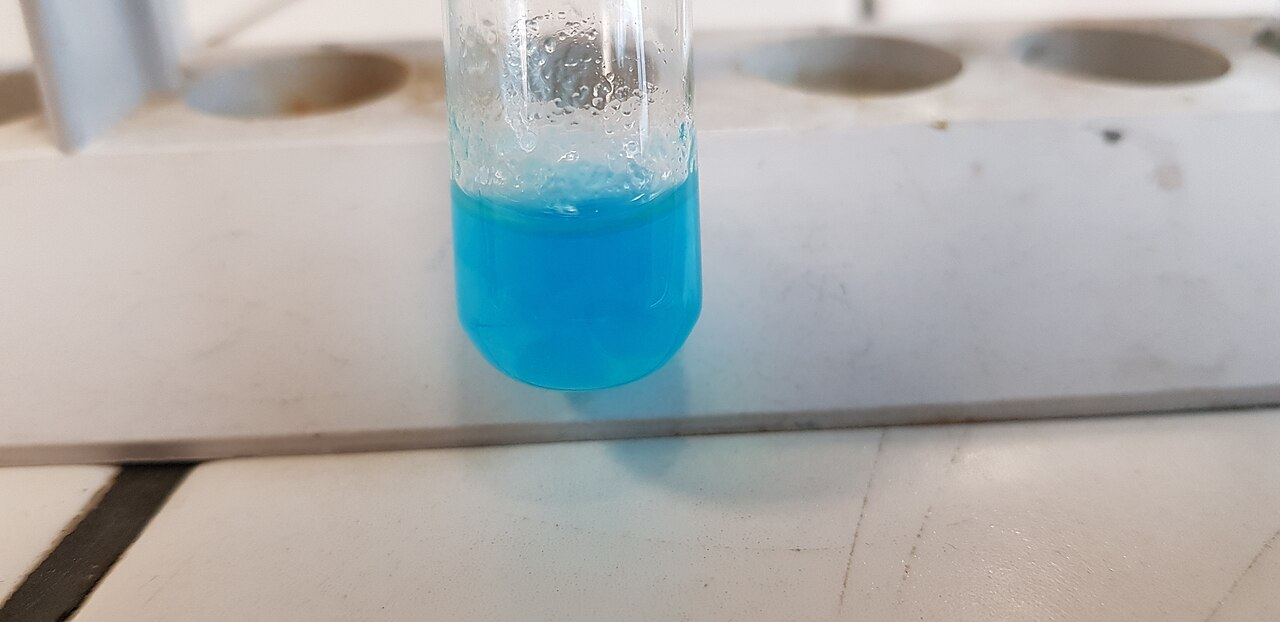
\includegraphics[height=4.2cm]{images/book2/copper-hydroxide.jpg}\hspace{0.6em}%
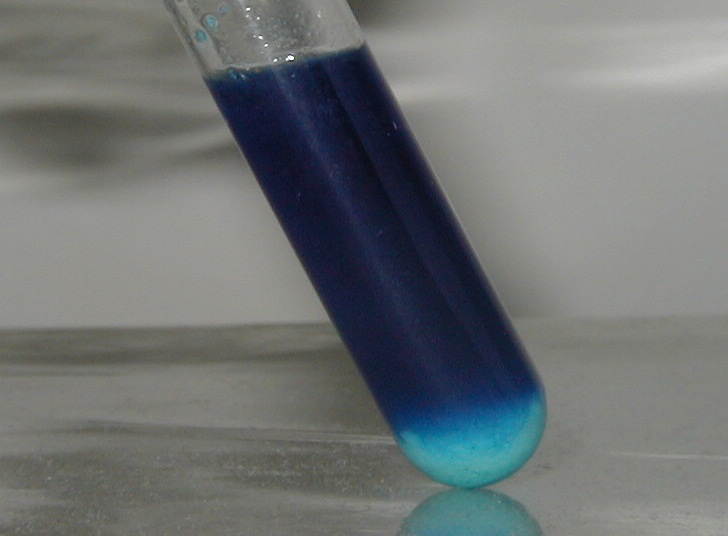
\includegraphics[height=4.2cm]{images/book2/copper-ammine.jpg}

{\small बाएँ: हल्के नीले कॉपर(II) हाइड्रॉक्साइड का निलंबन
(छायाचित्र: ऐल्वी16, CC BY 4.0)। दाएँ: और अमोनिया डालने पर ठोस
गहरे नीले टेट्राऐम्मीनकॉपर(II) आयन में घुल जाता है; कुछ बिना घुला
हाइड्रॉक्साइड अब भी नली की तली में है (छायाचित्र: केमिकलइंटरेस्ट,
सार्वजनिक अधिकार-क्षेत्र)। दोनों विकिमीडिया कॉमन्स।}
\end{omfigure}

\section{संकुल और लिगैंड}

\begin{definition}[संकुल, केंद्रीय परमाणु, लिगैंड]\label{def:b1:complexation:complex}
\emph{संकुल}\index{संकुल} ऐसी स्पीशीज़ है जो एक \emph{केंद्रीय
परमाणु}\index{केंद्रीय परमाणु} या आयन से बनी होती है, प्रायः \omterm{def:b1:lewis-resonance-vsepr:lewis-acid}{लुइस अम्ल} की तरह
व्यवहार करने वाला कोई धातु धनायन, जो \omterm{def:b1:lewis-resonance-vsepr:lewis-acid}{लुइस क्षारकों} की तरह व्यवहार करने वाले अणुओं या आयनों से
\omterm{def:b1:lewis-resonance-vsepr:lewis-acid}{उपसहसंयोजी आबंधों} द्वारा बँधा होता है; इन्हें \emph{लिगैंड}\index{लिगैंड} कहते हैं। इसका सूत्र
वर्ग कोष्ठक में, उसके कुल आवेश के साथ, लिखा जाता है: $[\ce{Cu(NH3)4}]^{2+}$,
$[\ce{Fe(CN)6}]^{4-}$, $[\ce{Ag(NH3)2}]^{+}$, $[\ce{FeSCN}]^{2+}$।
\end{definition}

\omterm{def:b1:complexation:complex}{संकुल} का आवेश केंद्रीय आयन और \omterm{def:b1:complexation:complex}{लिगैंडों} के आवेशों का योग
है: $\mathrm{Fe^{2+}}$ और छह \ce{CN-} मिलकर
$[\ce{Fe(CN)6}]^{4-}$ बनाते हैं। \omterm{def:b1:complexation:complex}{लिगैंड} के पास कम-से-कम एक \omterm{def:b1:lewis-resonance-vsepr:lewis}{एकाकी युग्म} होना चाहिए: \ce{NH3},
\ce{H2O}, \ce{OH-}, \ce{Cl-}, \ce{CN-}, \ce{SCN-} (S या N से बँधा)।
पानी में हर धातु आयन वास्तव में पहले से ही एक \omterm{def:b1:complexation:complex}{संकुल} है जिसमें पानी के
अणु \omterm{def:b1:complexation:complex}{लिगैंड} हैं, $[\ce{Cu(H2O)6}]^{2+}$ या $[\ce{Fe(H2O)6}]^{3+}$;
कोई दूसरा \omterm{def:b1:complexation:complex}{संकुल} बनाने का अर्थ है उन पानी के अणुओं का दूसरे
\omterm{def:b1:complexation:complex}{लिगैंडों} से विनिमय, और पानी के \omterm{def:b1:complexation:complex}{लिगैंड} सूत्रों में छोड़ दिए जाते हैं, जैसे जलयोजित प्रोटॉन
के लिए \ce{H3O+} लिखा जाता है।

\begin{omfigure}
\begin{tikzpicture}[font=\small, line cap=round]
  % [Ag(NH3)2]+ : linear
  \begin{scope}
    \node (ag) at (0,0) {\ce{Ag}};
    \node (n1) at (-1.2,0) {\ce{H3N}};
    \node (n2) at (1.2,0) {\ce{NH3}};
    \draw[thick] (n1) -- (ag) -- (n2);
    \node at (0,-1.75) {$[\ce{Ag(NH3)2}]^{+}$, रैखिक};
  \end{scope}
  % [Cu(NH3)4]2+ : square plane in perspective
  \begin{scope}[xshift=4.3cm, every node/.style={fill=white, inner sep=1.5pt}]
    \node (cu) at (0,0) {\ce{Cu}};
    \node (a) at (-1.45,-0.5) {\ce{H3N}};
    \node (b) at (1.45,0.5) {\ce{NH3}};
    \node (c) at (0.85,-0.9) {\ce{NH3}};
    \node (d) at (-0.85,0.9) {\ce{H3N}};
    \begin{pgfonlayer}{background}
    \draw[gray, dashed] (a.center) -- (c.center) -- (b.center) -- (d.center) -- cycle;
    \end{pgfonlayer}
    \draw[thick] (cu) -- (a); \draw[thick] (cu) -- (b);
    \draw[thick] (cu) -- (c); \draw[thick] (cu) -- (d);
    \node at (0,-1.75) {$[\ce{Cu(NH3)4}]^{2+}$, वर्ग समतलीय};
  \end{scope}
  % [Fe(CN)6]4- : octahedron
  \begin{scope}[xshift=9.2cm, every node/.style={fill=white, inner sep=1.5pt}]
    \node (fe) at (0,0) {\ce{Fe}};
    \node (t) at (0,1.3) {\ce{CN}};
    \node (u) at (0,-1.3) {\ce{CN}};
    \node (l) at (-1.45,-0.45) {\ce{NC}};
    \node (r) at (1.45,0.45) {\ce{CN}};
    \node (f) at (0.8,-0.8) {\ce{CN}};
    \node (k) at (-0.8,0.8) {\ce{NC}};
    \begin{pgfonlayer}{background}
    \draw[gray, dashed] (l.center) -- (f.center) -- (r.center) -- (k.center) -- cycle;
    \end{pgfonlayer}
    \foreach \x in {t,u,l,r,f,k} \draw[thick] (fe) -- (\x);
    \node at (0,-1.75) {$[\ce{Fe(CN)6}]^{4-}$, अष्टफलकीय};
  \end{scope}
\end{tikzpicture}

{\small तीन \omterm{def:b1:complexation:complex}{संकुल} और उनकी आकृतियाँ। हर रेखा \omterm{def:b1:complexation:complex}{लिगैंड} के \omterm{def:b1:lewis-resonance-vsepr:lewis}{एकाकी युग्म}
(अमोनिया का N, सायनाइड का C) से धातु आयन तक एक \omterm{def:b1:lewis-resonance-vsepr:lewis-acid}{उपसहसंयोजी
आबंध} है; डैश रेखाएँ चार \omterm{def:b1:complexation:complex}{लिगैंडों} का वर्ग दर्शाती हैं। \omterm{def:b1:complexation:complex}{संकुलों} की
आकृतियों की व्याख्या द्वितीय वर्ष के खंड में की गई है।}
\end{omfigure}

\begin{definition}[बहुदंतुर लिगैंड, कीलेट]\label{def:b1:complexation:chelate}
जो \omterm{def:b1:complexation:complex}{लिगैंड} एक ही केंद्रीय आयन से अपने कई परमाणुओं द्वारा एक साथ बँधता है,
वह \emph{बहुदंतुर लिगैंड}\index{बहुदंतुर लिगैंड} है; वह
\omterm{def:b1:complexation:complex}{संकुल} जो यह बनाता है, जिसमें \omterm{def:b1:complexation:complex}{लिगैंड} धातु आयन के चारों ओर वलय बंद करता है,
\emph{कीलेट}\index{कीलेट} है। एथिलीनडाइऐमीन
\ce{H2N-CH2-CH2-NH2} दो N परमाणुओं से बँधता है, ऑक्ज़ेलेट आयन
\ce{C2O4^2-} दो O परमाणुओं से, और एथिलीनडाइऐमीनटेट्राऐसीटेट आयन
(\emph{ईडीटीए}, जिसे \ce{Y^4-} लिखा जाता है) दो N और चार O परमाणुओं से।
\end{definition}

\begin{omfigure}
\setchemfig{atom sep=1.9em}
\chemfig{N(-[3]-[2]C(=[1]O)-[3]O^{-})(-[5]-[6]C(=[7]O)-[5]O^{-})-[0]-[0]N(-[1]-[2]C(=[3]O)-[1]O^{-})(-[7]-[6]C(=[5]O)-[7]O^{-})}
\hspace{2.2em}
\begin{tikzpicture}[font=\small, baseline=(ca.base)]
  \node[circle, draw, thick, fill=omDef!12, inner sep=1.5pt] (ca) at (0,0) {\ce{Ca}};
  \node (n1) at (-1.15,-0.35) {N};
  \node (n2) at (0.55,-0.6) {N};
  \node (o1) at (0,1.35) {O};
  \node (o2) at (0,-1.35) {O};
  \node (o3) at (1.15,0.35) {O};
  \node (o4) at (-0.55,0.6) {O};
  \foreach \x in {n1,n2,o1,o2,o3,o4} \draw[thick, omDef] (ca) -- (\x);
  \draw[omProp, thick] (n1) .. controls (-0.57,-0.95) .. (n2);
  \draw[omProp, thick] (n1) .. controls (-1.05,0.95) .. (o1);
  \draw[omProp, thick] (n1) .. controls (-1.5,0.25) .. (o4);
  \draw[omProp, thick] (n2) .. controls (0.5,-1.6) .. (o2);
  \draw[omProp, thick] (n2) .. controls (1.5,-0.3) .. (o3);
\end{tikzpicture}

{\small बाएँ: ईडीटीए आयन \ce{Y^4-}, अपने दो N परमाणुओं और चार
कार्बॉक्सिलेट समूहों के साथ। दाएँ: कैल्सियम--ईडीटीए \omterm{def:b1:complexation:chelate}{कीलेट} $[\ce{CaY}]^{2-}$,
व्यवस्थात्मक रूप में: छह दाता परमाणु (नीले आबंध) आयन के चारों ओर एक अष्टफलक
के कोनों पर हैं, दोनों N परमाणु अगल-बगल, और \omterm{def:b1:complexation:complex}{लिगैंड} की कार्बन
श्रृंखलाएँ (नारंगी) पाँच-पाँच परमाणुओं के पाँच वलय बंद करती हैं, जो
\omterm{def:b1:complexation:chelate}{कीलेट} वलय हैं।}
\end{omfigure}

ईडीटीए आयन कैल्सियम आयन को इतनी दृढ़ता से थामता है कि वह पानी की कठोरता के
अनुमापन का अभिकर्मक है (\cref{ch:b1:titration-methods})।

\section{विरचन और वियोजन स्थिरांक}

\begin{definition}[विरचन और वियोजन स्थिरांक]\label{def:b1:complexation:formation-constant}
किसी केंद्रीय आयन M और \omterm{def:b1:complexation:complex}{लिगैंड} L के लिए (आवेश छोड़ दिए गए हैं)
$\mathrm{ML}_n$ का \emph{समग्र
विरचन स्थिरांक}\index{समग्र विरचन स्थिरांक} वह स्थिरांक $\beta_n$ है जो
$\mathrm{M} + n\,\mathrm{L} \rightleftharpoons \mathrm{ML}_n$ का है,
\[
  \beta_n = \frac{[\mathrm{ML}_n]}{[\mathrm{M}][\mathrm{L}]^n} .
\]
\emph{क्रमिक विरचन स्थिरांक}\index{क्रमिक विरचन स्थिरांक}
$K_i$ एक \omterm{def:b1:complexation:complex}{लिगैंड} जुड़ने का स्थिरांक है,
$\mathrm{ML}_{i-1} + \mathrm{L} \rightleftharpoons \mathrm{ML}_i$।
\emph{वियोजन स्थिरांक}\index{वियोजन स्थिरांक}
उसका व्युत्क्रम है, $K_d = 1/K_i$, और $\mathrm{p}K_d = \log K_i$, ताकि
\omterm{def:b1:complexation:complex}{संकुल}/\omterm{def:b1:complexation:complex}{लिगैंड} युग्म का वर्णन ठीक \omterm{def:b1:predominant-reaction:bronsted}{अम्ल--क्षारक युग्म} की तरह हो,
जिसमें प्रोटॉन के स्थान पर \omterm{def:b1:complexation:complex}{लिगैंड} हो।
\end{definition}

\begin{proposition}[समग्र और क्रमिक स्थिरांक]\label{prop:b1:complexation:beta-k}
$\beta_n = K_1 K_2 \cdots K_n$, अर्थात्
$\log\beta_n = \sum_{i=1}^n \log K_i$ और $\log K_i = \log\beta_i -
\log\beta_{i-1}$ ($\beta_0 = 1$ के साथ)।
\end{proposition}

\begin{proof}
M से $\mathrm{ML}_n$ का विरचन $n$ क्रमिक
योगों का योग है; अभिक्रियाओं के योग का स्थिरांक उनके
स्थिरांकों का गुणनफल होता है (\cref{ch:b1:extent-q-and-k})। सीधे:
$K_1 K_2\cdots K_n = \frac{[\mathrm{ML}]}{[\mathrm{M}][\mathrm{L}]}
\frac{[\mathrm{ML_2}]}{[\mathrm{ML}][\mathrm{L}]}\cdots
\frac{[\mathrm{ML}_n]}{[\mathrm{ML}_{n-1}][\mathrm{L}]}$, और
बीच की सांद्रताएँ कट जाती हैं।
\end{proof}

\begin{omfigure}
\begin{tabular}{lll}
\hline
\omterm{def:b1:complexation:complex}{संकुल} & $\log\beta_n$ & $\log K_i$ \\
\hline
$[\ce{Cu(NH3)_n}]^{2+}$, $n = 1$ से 4 & 4.10, 7.51, 10.33, 12.36 & 4.10, 3.41, 2.82, 2.03 \\
$[\ce{Ag(NH3)_n}]^{+}$, $n = 1, 2$ & 3.32, 7.22 & 3.32, 3.90 \\
$[\ce{Zn(OH)4}]^{2-}$ & $\log\beta_4 = 14.45$ & \\
$[\ce{FeSCN}]^{2+}$, $[\ce{FeF}]^{2+}$ & 2.96; 6.85 & \\
$[\ce{CaY}]^{2-}$, $[\ce{MgY}]^{2-}$, $[\ce{NiY}]^{2-}$ & 12.69, 10.90, 20.54 & \\
\hline
\end{tabular}

\smallskip
{\small \qty{25}{\celsius} पर विरचन स्थिरांक। ऐम्मीन, हाइड्रॉक्सो,
थायोसायनेटो और फ़्लुओरो स्थिरांक सारणीबद्ध मानक विरचन
गिब्ज़ ऊर्जाओं से परिकलित हैं; ईडीटीए के स्थिरांक शून्य आयनिक सामर्थ्य पर
समालोचनात्मक रूप से चयनित मान हैं, और नीचे प्रयुक्त ईडीटीए के $\mathrm{p}K_a$,
2.23, 3.15, 6.80 और 11.24, भी।}
% ledger: dfg:Cu2+_ao, dfg:CuNH32+_ao, dfg:Cu_NH322+_ao, dfg:Cu_NH332+_ao, dfg:Cu_NH342+_ao, dfg:NH3_ao (computed in figdata/bachelor-1/aqueous-constants.py)
% ledger: dfg:Ag+_ao, dfg:AgNH3+_ao, dfg:Ag_NH32+_ao, dfg:Fe3+_ao, dfg:SCN-_ao, dfg:FeSCN2+_ao, dfg:F-_ao, dfg:FeF2+_ao (computed, same script)
% ledger: logb:Ca-edta, logb:Mg-edta, logb:Ni-edta, pka:edta1, pka:edta2, pka:edta3, pka:edta4
\end{omfigure}

कॉपर ऐम्मीनों के क्रमिक स्थिरांक घटते जाते हैं, $K_1 > K_2 > K_3
> K_4$: जुड़ने वाला हर अमोनिया अणु कम स्थल छोड़ता है और \omterm{def:b1:complexation:complex}{संकुल} को
अगले अणु के लिए थोड़ा कम आतुर बनाता है। यही सामान्य क्रम है।
सिल्वर एक अपवाद है: $K_2 > K_1$, जिसके परिणाम
सप्ताहांत समस्या में निकाले गए हैं।

\section{pL में प्रभाविता}

\begin{definition}[pL पैमाना]\label{def:b1:complexation:pl-diagram}
किसी \omterm{def:b1:complexation:complex}{लिगैंड} L के लिए $\mathrm{pL} = -\log[\mathrm{L}]$, जहाँ $[\mathrm{L}]$
मुक्त \omterm{def:b1:complexation:complex}{लिगैंड} की सांद्रता है। \emph{pL पैमाना}\index{pL पैमाना}
pL का एक अक्ष है जिस पर केंद्रीय आयन और उसके \omterm{def:b1:complexation:complex}{संकुलों} के प्रभाविता क्षेत्र
बनाए जाते हैं, जैसे अम्लों और क्षारकों के क्षेत्र
pH अक्ष पर बनाए जाते हैं।
\end{definition}

\begin{proposition}[pL में सीमाएँ]\label{prop:b1:complexation:pl-boundaries}
युग्म $\mathrm{ML}_i/\mathrm{ML}_{i-1}$ के लिए,
\[
  \mathrm{pL} = \log K_i + \log\frac{[\mathrm{ML}_{i-1}]}{[\mathrm{ML}_i]} ,
\]
इसलिए $\mathrm{ML}_{i-1}$, $\mathrm{pL} > \log K_i$ के लिए प्रभावी है और
$\mathrm{ML}_i$, $\mathrm{pL} < \log K_i$ के लिए। जब $\log K_i$, $i$ के साथ
घटते हैं, तो आरेख क्षेत्रों का एक क्रम होता है: छोटे pL (अधिक \omterm{def:b1:complexation:complex}{लिगैंड}) पर $\mathrm{ML}_n$,
फिर $\mathrm{ML}_{n-1}$, और बड़े pL पर M तक।
\end{proposition}

\begin{proof}
$K_i = [\mathrm{ML}_i]/([\mathrm{ML}_{i-1}][\mathrm{L}])$ का लघुगणक लीजिए:
$\log K_i = \log\frac{[\mathrm{ML}_i]}{[\mathrm{ML}_{i-1}]} + \mathrm{pL}$।
दोनों रूप $\mathrm{pL} = \log K_i$ पर बराबर होते हैं, और अनुपात pL की
हर इकाई पर दस के गुणक से बदलता है। $\mathrm{ML}_i$ का क्षेत्र
$\log K_{i+1}$ और $\log K_i$ के बीच है, जो केवल तभी अस्तित्व में होता है जब $\log K_{i+1} < \log
K_i$।
\end{proof}

\begin{method}[pL आरेख बनाना]\label{met:b1:complexation:pl-diagram}
\begin{enumerate}
  \item $\log\beta_n$ से क्रमिक $\log K_i$ परिकलित कीजिए।
  \item यदि वे घटते हैं, तो हर एक को pL अक्ष पर उसकी सीमा पर रखिए:
        सबसे अधिक \omterm{def:b1:complexation:complex}{लिगैंडों} वाला \omterm{def:b1:complexation:complex}{संकुल} बाईं ओर (छोटा pL), मुक्त
        आयन दाईं ओर।
  \item यदि कोई $\log K_{i+1} > \log K_i$, तो \omterm{def:b1:complexation:complex}{संकुल} $\mathrm{ML}_i$ का
        कोई क्षेत्र नहीं होता: वह स्वयं से अभिक्रिया करके $\mathrm{ML}_{i-1}$ और
        $\mathrm{ML}_{i+1}$ बन जाता है। उसे हटाइए और
        $\mathrm{ML}_{i-1}$ और $\mathrm{ML}_{i+1}$ के बीच
        $\frac12(\log K_i + \log K_{i+1})$ पर एक ही सीमा बनाइए।
\end{enumerate}
\end{method}

\begin{omfigure}
\begin{tikzpicture}
\begin{axis}[
  width=0.78\linewidth, height=5.2cm, xmin=0, xmax=7, ymin=0, ymax=1.05,
  axis x line=bottom, axis y line=left, xlabel={$\mathrm{pNH_3}$},
  ylabel={कॉपर का अंश},
  tick label style={font=\small}, label style={font=\small}]
\addplot[omThm, thick] table[x=pL, y=M] {figdata/out/bachelor-1-ammine-distribution-copper.dat};
\addplot[omProp, thick] table[x=pL, y=ML] {figdata/out/bachelor-1-ammine-distribution-copper.dat};
\addplot[omMeth, thick] table[x=pL, y=ML2] {figdata/out/bachelor-1-ammine-distribution-copper.dat};
\addplot[black!60, thick] table[x=pL, y=ML3] {figdata/out/bachelor-1-ammine-distribution-copper.dat};
\addplot[omDef, very thick] table[x=pL, y=ML4] {figdata/out/bachelor-1-ammine-distribution-copper.dat};
\node[omDef, font=\small, anchor=west] at (axis cs:0.15,0.78) {$n = 4$};
\node[black!60, font=\small] at (axis cs:2.42,0.63) {3};
\node[omMeth, font=\small] at (axis cs:3.12,0.55) {2};
\node[omProp, font=\small] at (axis cs:3.76,0.58) {1};
\node[omThm, font=\small, anchor=east] at (axis cs:6.9,0.84) {\ce{Cu^2+}};
\end{axis}
\end{tikzpicture}

\begin{tikzpicture}[font=\small, x=1.25cm]
  \draw[->, thick] (0,0) -- (7.2,0) node[right] {$\mathrm{pNH_3}$};
  \foreach \x/\l in {2.03/2.03, 2.82/2.82, 3.41/3.41, 4.10/4.10}
    \draw (\x,0.12) -- (\x,-0.12) node[below] {\l};
  \node[above] at (1.0,0.08) {$[\ce{Cu(NH3)4}]^{2+}$};
  \node[above, font=\scriptsize] at (2.42,0.08) {3};
  \node[above, font=\scriptsize] at (3.12,0.08) {2};
  \node[above, font=\scriptsize] at (3.76,0.08) {1};
  \node[above] at (5.6,0.08) {\ce{Cu^2+}};
  \begin{scope}[yshift=-1.25cm]
  \draw[->, thick] (0,0) -- (7.2,0) node[right] {$\mathrm{pNH_3}$};
  \draw (3.61,0.12) -- (3.61,-0.12) node[below] {3.61};
  \draw[dotted] (3.32,0.3) -- (3.32,-0.1); \draw[dotted] (3.90,0.3) -- (3.90,-0.1);
  \node[above] at (1.6,0.08) {$[\ce{Ag(NH3)2}]^{+}$};
  \node[above] at (5.4,0.08) {\ce{Ag+}};
  \end{scope}
\end{tikzpicture}

{\small ऊपर: \ce{Cu^2+} के रूप में और
$[\ce{Cu(NH3)_n}]^{2+}$ ($n = 1$ से 4) के रूप में उपस्थित कॉपर(II) के अंश,
$\mathrm{pNH_3}$ के सापेक्ष। बीच में:
कॉपर ऐम्मीनों का \omterm{def:b1:predominant-reaction:predominance}{प्रभाविता आरेख}, सीमाएँ
$\log K_i$ पर। नीचे: सिल्वर, जहाँ $\log K_2 = 3.90 > \log K_1 = 3.32$
(बिंदुदार): $[\ce{AgNH3}]^{+}$ का कोई क्षेत्र नहीं है और एक ही सीमा
$\frac12\log\beta_2 = 3.61$ पर है।}
\end{omfigure}

\begin{example}[\texorpdfstring{\qty{0.010}{mol/L}}{0.010 mol/L} अमोनिया में कॉपर]\label{ex:b1:complexation:cu}
मुक्त $[\ce{NH3}] = \qty{0.010}{mol/L}$ पर $\mathrm{pNH_3} = 2.0$,
$[\ce{Cu(NH3)3}]^{2+}$ के क्षेत्र में है पर
$[\ce{Cu(NH3)4}]^{2+}$ के साथ सीमा 2.03 के पास: दोनों लगभग बराबर हैं। अंश
$\beta_n[\ce{NH3}]^n = 10^{\log\beta_n - 2n}$ के समानुपाती हैं, अर्थात्
$1 : 10^{2.10} : 10^{3.51} : 10^{4.33} : 10^{4.36}$, इसलिए \qty{48}{\percent}
$[\ce{Cu(NH3)4}]^{2+}$, \qty{45}{\percent} $[\ce{Cu(NH3)3}]^{2+}$,
\qty{7}{\percent} $[\ce{Cu(NH3)2}]^{2+}$ और मुक्त \ce{Cu^2+} लगभग कुछ नहीं।
\end{example}

\section{प्रतिस्पर्धाएँ}

किसी \omterm{def:b1:complexation:complex}{लिगैंड} पर दो धातु आयन दावा कर सकते हैं, किसी धातु आयन पर दो \omterm{def:b1:complexation:complex}{लिगैंड},
और दोनों अवक्षेपण और अम्ल--क्षारक साम्यों में भी लगे होते हैं।
हर प्रतिस्पर्धा एक और अभिक्रिया है जिसका स्थिरांक पहले से ज्ञात
स्थिरांकों को जोड़कर बनता है; तब \cref{ch:b1:predominant-reaction} की
प्रधान-अभिक्रिया विधि बिना बदले लागू होती है।

\begin{example}[आयरन(III) के लिए दो लिगैंड]\label{ex:b1:complexation:scn-f}
आयरन(III) विलयन में थायोसायनेट की एक बूँद रक्त-लाल
$[\ce{FeSCN}]^{2+}$ देती है; फ़्लुओराइड आयन इसे रंगहीन कर देते हैं:
\[
  [\ce{FeSCN}]^{2+} + \ce{F-} \rightleftharpoons [\ce{FeF}]^{2+} + \ce{SCN-},
  \qquad K = \frac{\beta(\ce{FeF})}{\beta(\ce{FeSCN})} = 10^{6.85 - 2.96} =
  10^{3.89} .
\]
अधिक प्रबल \omterm{def:b1:complexation:complex}{संकुल} (बड़ा $\beta$) धातु आयन ले लेता है, ठीक वैसे ही जैसे
अधिक \omterm{def:b1:predominant-reaction:strong-acid}{प्रबल अम्ल} अपना प्रोटॉन अधिक \omterm{def:b1:predominant-reaction:strong-acid}{प्रबल क्षारक} को देता है।
\end{example}

\begin{proposition}[संकुलन बनाम अवक्षेपण]\label{prop:b1:complexation:competition-precipitation}
कोई ठोस MX किसी \omterm{def:b1:complexation:complex}{लिगैंड} L में
$\mathrm{MX(s)} + n\,\mathrm{L} \rightleftharpoons \mathrm{ML}_n + \mathrm{X}$ द्वारा घुलता है,
जिसका स्थिरांक $K = \beta_n K_s$ है। यदि विलयन में M का एकमात्र रूप \omterm{def:b1:complexation:complex}{संकुल} हो
और मुक्त \omterm{def:b1:complexation:complex}{लिगैंड} की सांद्रता $[\mathrm{L}]$ हो, तो
\omterm{def:b1:precipitation:solubility}{विलेयता} $s = \sqrt{K}\,[\mathrm{L}]^{n/2}$ है।
\end{proposition}

\begin{proof}
अभिक्रिया घुलन (स्थिरांक $K_s$) और
$\mathrm{ML}_n$ के विरचन ($\beta_n$) का योग है। संतृप्ति पर $[\mathrm{ML}_n]
= [\mathrm{X}] = s$ और $K = s^2/[\mathrm{L}]^n$।
\end{proof}

\begin{method}[संकुलन द्वारा अवक्षेप को घोलना]\label{met:b1:complexation:dissolve-precipitate}
\begin{enumerate}
  \item \omterm{def:b1:complexation:complex}{संकुल} में घुलने की अभिक्रिया लिखिए और
        $K = \beta_n K_s$ परिकलित कीजिए।
  \item यदि $K$ बड़ा है, तो जब तक पर्याप्त \omterm{def:b1:complexation:complex}{लिगैंड} उपस्थित हो, घुलन \omterm{def:b1:extent-q-and-k:quantitative}{मात्रात्मक} है;
        यदि छोटा है, तो ठोस की उस मात्रा को घोलने के लिए आवश्यक मुक्त \omterm{def:b1:complexation:complex}{लिगैंड}
        सांद्रता परिकलित कीजिए:
        $[\mathrm{L}]^n = s^2/K$।
  \item डाले जाने वाले कुल \omterm{def:b1:complexation:complex}{लिगैंड} को प्राप्त करने के लिए \omterm{def:b1:complexation:complex}{संकुल} में बँधा \omterm{def:b1:complexation:complex}{लिगैंड}, $n s$,
        जोड़िए।
  \item जाँचिए कि मुक्त धातु आयन नगण्य है: $[\mathrm{M}] = K_s/s
        \ll s$।
\end{enumerate}
\end{method}

अमोनिया के साथ सिल्वर क्लोराइड ($K = 10^{7.22 - 9.75} = 10^{-2.53}$)
मध्यम सांद्र विलयन में घुल जाता है जबकि सिल्वर आयोडाइड
($K = 10^{-8.85}$) नहीं: सप्ताहांत समस्या इसका उपयोग
हैलाइडों को अलग पहचानने में करती है।

\begin{proposition}[संकुलन बनाम अम्लता]\label{prop:b1:complexation:ligand-acidity}
यदि \omterm{def:b1:complexation:complex}{लिगैंड} एक क्षारक $\mathrm{L}$ है, जो किसी अम्ल $\mathrm{HL}$ का क्षारक है (और
संभवतः अधिक प्रोटॉनित रूप भी हैं), तो धातु से न बँधे \omterm{def:b1:complexation:complex}{लिगैंड} का केवल
भिन्न $[\mathrm{L}]/c_L =
1/\alpha$ उपलब्ध होता है, जहाँ
\[
  \alpha = 1 + \frac{[\ce{H3O+}]}{K_{an}} + \frac{[\ce{H3O+}]^2}{K_{an}K_{a(n-1)}}
  + \cdots
\]
($K_{an}$ अंतिम \omterm{def:b1:predominant-reaction:acidity-constant}{अम्लता स्थिरांक} है)। किसी स्थिर pH पर तब संकुलन
ऐसा व्यवहार करता है मानो उसका स्थिरांक \emph{सशर्त} स्थिरांक
$\beta' = \beta/\alpha$ हो, जो pH जितना कम हो उतना छोटा होता है।
\end{proposition}

\begin{proof}
धातु से न बँधा \omterm{def:b1:complexation:complex}{लिगैंड} L, HL, \ce{H2L} आदि में
बँटा होता है, जहाँ $[\mathrm{HL}] = [\mathrm{L}][\ce{H3O+}]/K_{an}$ और
अगले रूपों के लिए इसी तरह के संबंध हैं (\cref{ch:b1:predominant-reaction})। योग करने पर $c_L = \alpha[\mathrm{L}]$ मिलता है,
और $\beta = [\mathrm{ML}]/([\mathrm{M}][\mathrm{L}]) =
\alpha[\mathrm{ML}]/([\mathrm{M}]c_L)$, इसलिए $[\mathrm{ML}]/([\mathrm{M}]c_L)
= \beta/\alpha$।
\end{proof}

pH 10 पर ईडीटीए के लिए $\alpha = 1 + 10^{11.24 - 10} + 10^{11.24 + 6.80 - 20}
= 18.4$, इसलिए कैल्सियम \omterm{def:b1:complexation:complex}{संकुल} $\log\beta' = 12.69 - 1.26 = 11.43$ बनाए रखता है;
pH 7 पर यह 8.24 तक गिर जाता है (\cref{exo:b1:complexation:9})। इसीलिए
ईडीटीए से कैल्सियम का अनुमापन pH 10 के अमोनिया बफ़र में किया जाता है।
अमोनिया भी एक क्षारक है: अम्ल में वह \ce{NH4+} बन जाता है, जिसके पास कोई \omterm{def:b1:lewis-resonance-vsepr:lewis}{एकाकी
युग्म} नहीं, और ऐम्मीन \omterm{def:b1:complexation:complex}{संकुल} टूट जाते हैं। क्लोराइड की उपस्थिति में
$[\ce{Ag(NH3)2}]^{+}$ में नाइट्रिक अम्ल मिलाने से सिल्वर क्लोराइड का सफ़ेद
अवक्षेप लौट आता है।

फ़ोटोग्राफ़िक स्थायीकारक सिल्वर आयन के एक दूसरे \omterm{def:b1:complexation:complex}{लिगैंड}, थायोसल्फ़ेट आयन
\ce{S2O3^2-}, के साथ यही करते हैं: वे उस सिल्वर हैलाइड को घोल देते हैं जिसे
प्रकाश ने नहीं छुआ, ताकि चित्र और काला न पड़े। उसके
स्थिरांक इस खंड के आँकड़ों में नहीं हैं; अमोनिया सिल्वर क्लोराइड के साथ यही
रसायन दिखाता है।

\section{अभ्यास}

\begin{exercise}[$\star$]\label{exo:b1:complexation:1}
हर \omterm{def:b1:complexation:complex}{संकुल} के लिए केंद्रीय आयन, उसका आवेश, \omterm{def:b1:complexation:complex}{लिगैंड} और वह
परमाणु बताइए जिसके द्वारा हर \omterm{def:b1:complexation:complex}{लिगैंड} बँधता है: $[\ce{Cu(NH3)4}]^{2+}$,
$[\ce{Fe(CN)6}]^{4-}$, $[\ce{Fe(CN)6}]^{3-}$, $[\ce{Ag(NH3)2}]^{+}$,
$[\ce{FeSCN}]^{2+}$, $[\ce{Zn(OH)4}]^{2-}$, $[\ce{CaY}]^{2-}$।
\end{exercise}

\begin{exercise}[$\star$]\label{exo:b1:complexation:2}
कॉपर ऐम्मीनों के $\log\beta_n$ से चारों $\log K_i$
और चारों $\mathrm{p}K_d$ परिकलित कीजिए। वह वियोजन अभिक्रिया लिखिए जिससे
अंतिम $\mathrm{p}K_d$ संबंधित है।
\end{exercise}

\begin{exercise}[$\star$]\label{exo:b1:complexation:3}
कॉपर ऐम्मीनों का pL आरेख बनाइए। $[\ce{NH3}] = 1.0$, \num{3.2e-3}, \num{3.2e-4} और
\qty{1.0e-5}{mol/L} पर कौन-सी कॉपर स्पीशीज़
प्रभावी है?
\end{exercise}

\begin{exercise}[$\star$]\label{exo:b1:complexation:4}
एक विलयन में \qty{1.0e-3}{mol/L} आयरन(III) और
\qty{0.10}{mol/L} थायोसायनेट है। बँधे थायोसायनेट को नगण्य मानकर, आयरन का
कितना भिन्न $[\ce{FeSCN}]^{2+}$ के रूप में उपस्थित है?
\end{exercise}

\begin{exercise}[$\star\star$]\label{exo:b1:complexation:5}
सिद्ध कीजिए कि किसी धातु आयन M और उसके \omterm{def:b1:complexation:complex}{संकुलों}
$\mathrm{ML}_n$ के विलयन में $\mathrm{ML}_n$ का अंश
$\beta_n[\mathrm{L}]^n / \sum_{k} \beta_k[\mathrm{L}]^k$ है। दिखाइए कि,
यदि केवल $\mathrm{ML}_{i-1}$, $\mathrm{ML}_i$ और $\mathrm{ML}_{i+1}$
उल्लेखनीय मात्रा में उपस्थित हों, तो $\mathrm{ML}_i$ का अंश
वहाँ सबसे बड़ा है जहाँ $[\mathrm{ML}_{i-1}] = [\mathrm{ML}_{i+1}]$, अर्थात्
$\mathrm{pL} = \frac12(\log K_i + \log K_{i+1})$ पर, और
$[\ce{Cu(NH3)2}]^{2+}$ के लिए यह pNH3 परिकलित कीजिए।
\end{exercise}

\begin{exercise}[$\star\star$]\label{exo:b1:complexation:6}
\cref{exo:b1:complexation:4} के लाल विलयन में सोडियम फ़्लुओराइड
तब तक डाला जाता है जब तक $[\ce{F-}] = \qty{0.010}{mol/L}$ (मुक्त) न हो जाए। \omterm{def:b1:complexation:complex}{लिगैंडों} के
विनिमय का स्थिरांक और अनुपात $[\ce{FeF^2+}]/[\ce{FeSCN^2+}]$ परिकलित कीजिए।
क्या दिखाई देता है?
\end{exercise}

\begin{exercise}[$\star\star$]\label{exo:b1:complexation:7}
$[\ce{MgY}]^{2-}$ के विलयन में बराबर मात्रा में कैल्सियम आयन
डाले जाते हैं। विनिमय अभिक्रिया लिखिए, उसका स्थिरांक परिकलित कीजिए और
मुक्त हुए मैग्नीशियम का भिन्न भी।
\end{exercise}

\begin{exercise}[$\star\star$]\label{exo:b1:complexation:8}
सिल्वर ऑक्साइड \ce{Ag2O} एक भूरा ठोस है: \ce{Ag2O(s) + H2O <=> 2Ag+ + 2OH-}
का $\mathrm{p}K = 15.43$ है। इसका अमोनिया में
$[\ce{Ag(NH3)2}]^{+}$ के रूप में घुलना लिखिए, स्थिरांक परिकलित कीजिए, और समझाइए कि
सिल्वर नाइट्रेट में थोड़ा अमोनिया डालने से बना भूरा
अवक्षेप और अमोनिया डालने पर क्यों घुल जाता है।
\end{exercise}

\begin{exercise}[$\star\star$]\label{exo:b1:complexation:9}
pH 10 और pH 7 पर $\alpha$ और सशर्त स्थिरांक $\log\beta'$ परिकलित कीजिए,
$[\ce{CaY}]^{2-}$ के लिए (\cref{prop:b1:complexation:ligand-acidity})। यदि कम-से-कम $10^{10}$ का
सशर्त स्थिरांक आवश्यक हो, तो उदासीन विलयन में
ईडीटीए से कैल्सियम का अनुमापन असंभव क्यों है?
\end{exercise}

\begin{exercise}[$\star\star\star$]\label{exo:b1:complexation:10}
कॉपर(II) ऑक्साइड \ce{CuO} वह ठोस है जिसमें कॉपर(II) हाइड्रॉक्साइड
रखे रहने पर बदल जाता है; \ce{CuO(s) + H2O <=> Cu^2+ + 2OH-} का $\mathrm{p}K = 20.64$ है।
\begin{enumerate}
  \item \ce{CuO} का अमोनिया में
        $[\ce{Cu(NH3)4}]^{2+}$ के रूप में घुलना लिखिए और उसका स्थिरांक परिकलित कीजिए।
  \item केवल \qty{1.0}{mol/L} अमोनिया में pH अमोनिया द्वारा तय होता है
        ($\mathrm{p}K_a(\ce{NH4+}) = 9.25$)। pH और
        घुले कॉपर की सांद्रता परिकलित कीजिए।
  \item यही प्रश्न अमोनिया और अमोनियम क्लोराइड के बफ़र में, दोनों
        \qty{1.0}{mol/L} पर। निष्कर्ष निकालिए।
\end{enumerate}
\end{exercise}

\begin{exercise}[$\star\star\star$]\label{exo:b1:complexation:11}
सिल्वर और अमोनिया।
\begin{enumerate}
  \item दिखाइए कि $[\ce{AgNH3}]^{+}$ स्वयं से अभिक्रिया करता है,
        \ce{2[AgNH3]+ <=> Ag+ + [Ag(NH3)2]+}, और स्थिरांक परिकलित कीजिए।
  \item सिल्वर का वह अधिकतम भिन्न परिकलित कीजिए जो कभी
        $[\ce{AgNH3}]^{+}$ के रूप में उपस्थित होता है, और वह pNH3 जहाँ ऐसा होता है।
\end{enumerate}
\end{exercise}

\begin{exercise}[$\star\star\star$]\label{exo:b1:complexation:12}
ईडीटीए का एक विलयन, उच्च pH पर \ce{Y^4-} का \qty{0.10}{mol/L}, कैल्सियम कार्बोनेट
की पपड़ी घोलने के लिए प्रयुक्त होता है।
\begin{enumerate}
  \item अभिक्रिया लिखिए और उसका स्थिरांक परिकलित कीजिए।
  \item एक लीटर कैल्सियम कार्बोनेट का कितना द्रव्यमान घोल सकता है?
  \item विलयन क्षारकीय क्यों होना चाहिए? (कार्बोनेट और ईडीटीए आयन
        दोनों क्षारक हैं।)
\end{enumerate}
\end{exercise}

\section{समस्या: अमोनिया और तीन सिल्वर हैलाइड}

\begin{problem}[{सप्ताहांत समस्या --- सिल्वर ऐम्मीन और उनके
उलटे स्थिरांक, सिल्वर क्लोराइड, ब्रोमाइड और आयोडाइड को
अमोनिया में घोलना, पुष्टि परीक्षण, और एक ग्राम सिल्वर क्लोराइड को घोलने वाली
न्यूनतम अमोनिया}]
\label{pb:b1:complexation:1}
एक विश्लेषक के पास सफ़ेद से पीले तक के तीन अवक्षेप हैं और उसे बताना है कि कौन-सा
सिल्वर का क्लोराइड, कौन-सा ब्रोमाइड और कौन-सा आयोडाइड है; फिर उसे
\qty{1.0}{g} सिल्वर क्लोराइड को \qty{1.00}{L} में यथासंभव कम
अमोनिया से घोलना है। \qty{25}{\celsius} पर आँकड़े: सिल्वर ऐम्मीनों के लिए $\log\beta_1 = 3.32$ और
$\log\beta_2 = 7.22$; $\mathrm{p}K_s$: \ce{AgCl}
9.75, \ce{AgBr} 12.27, \ce{AgI} 16.07; $\mathrm{p}K_a(\ce{NH4+}) = 9.25$;
मोलर द्रव्यमान \ce{AgCl} \qty{143.4}{g/mol}, \ce{AgBr} \qty{187.8}{g/mol},
\ce{AgI} \qty{234.8}{g/mol}।

\medskip
\noindent\textbf{भाग I --- सिल्वर ऐम्मीन।}
\begin{enumerate}
  \item $[\ce{AgNH3}]^{+}$ और
        $[\ce{Ag(NH3)2}]^{+}$ की विरचन अभिक्रियाएँ तथा $\beta_1$ और $\beta_2$ के व्यंजक लिखिए।
  \item $\log K_1$ और $\log K_2$ परिकलित कीजिए।
  \item इन दो सीमाओं के साथ सरल ढंग से pL आरेख बनाइए। इसमें क्या
        ग़लत है?
  \item $[\ce{AgNH3}]^{+}$ की स्वयं से अभिक्रिया लिखिए और
        उसका स्थिरांक परिकलित कीजिए।
  \item सही आरेख बनाइए; उसकी एकमात्र सीमा कहाँ है?
  \item $[\ce{NH3}] = \qty{0.10}{mol/L}$ पर
        $[\ce{Ag(NH3)2+}]/[\ce{Ag+}]$ परिकलित कीजिए।
  \item समग्र \omterm{def:b1:complexation:formation-constant}{वियोजन स्थिरांक} $\mathrm{p}K_d$ बताइए,
        $[\ce{Ag(NH3)2}]^{+}$ का।
\end{enumerate}

\medskip
\noindent\textbf{भाग II --- अमोनिया में सिल्वर क्लोराइड।}
\begin{enumerate}[resume]
  \item अमोनिया में \ce{AgCl} का घुलना लिखिए और उसका
        स्थिरांक परिकलित कीजिए।
  \item \omterm{def:b1:precipitation:solubility}{विलेयता} $s$ को मुक्त अमोनिया की
        सांद्रता के फलन के रूप में व्यक्त कीजिए और $[\ce{NH3}] = \qty{1.0}{mol/L}$ के लिए इसे परिकलित कीजिए।
  \item शुद्ध पानी की तुलना में \omterm{def:b1:precipitation:solubility}{विलेयता} कितनी बढ़ गई है?
  \item तब एक लीटर सिल्वर क्लोराइड का कितना द्रव्यमान घोलता है?
  \item जाँचिए कि मुक्त \ce{Ag+} नगण्य है।
  \item अब \qty{1.0}{mol/L} डाली गई कुल अमोनिया है। बँधी हुई
        अमोनिया को ध्यान में रखकर $s$ फिर से परिकलित कीजिए।
  \item अमोनिया एक क्षारक है; समझाइए कि इस विलयन में उसके प्रोटॉनन को नगण्य
        क्यों माना जा सकता है।
\end{enumerate}

\medskip
\noindent\textbf{भाग III --- ब्रोमाइड और आयोडाइड।}
\begin{enumerate}[resume]
  \item अमोनिया में \ce{AgBr} के घुलने का स्थिरांक परिकलित कीजिए।
  \item \qty{1.0}{mol/L} मुक्त अमोनिया में \ce{AgBr} की \omterm{def:b1:precipitation:solubility}{विलेयता}
        \unit{mol/L} और \unit{g/L} में परिकलित कीजिए।
  \item यही \ce{AgI} के लिए, \unit{mg/L} में।
  \item तीनों अवक्षेपों को पहचानने का एक तरीका निकालिए।
  \item \qty{1.00}{L} में \qty{1.0}{g}
        \ce{AgBr} घोलने के लिए मुक्त अमोनिया की कितनी सांद्रता चाहिए?
  \item यही \qty{1.0}{g} \ce{AgI} के लिए। टिप्पणी कीजिए।
\end{enumerate}

\medskip
\noindent\textbf{भाग IV --- एक ग्राम सिल्वर क्लोराइड।}
\begin{enumerate}[resume]
  \item सिल्वर क्लोराइड के अमोनियायुक्त विलयन में नाइट्रिक अम्ल
        मिलाया जाता है। समग्र अभिक्रिया लिखिए और उसका स्थिरांक परिकलित कीजिए। विश्लेषक
        क्या देखती है?
  \item \qty{1.00}{L} में \qty{1.0}{g}
        \ce{AgCl} घोलने के लिए मुक्त अमोनिया की कितनी सांद्रता चाहिए?
  \item \omterm{def:b1:complexation:complex}{संकुल} में कितनी अमोनिया बँधी है?
  \item जाँचिए कि इस विलयन में मुक्त \ce{Ag+} नगण्य है।
  \item \qty{1.00}{L} में \qty{1.0}{g} सिल्वर क्लोराइड घोलने वाली
        अमोनिया की न्यूनतम कुल सांद्रता क्या है?
\end{enumerate}
\end{problem}
